\documentclass[10pt,conference,compsocconf]{./IEEEtran} 
%\documentclass[10pt,conference]{IEEEtran} 

\usepackage{setspace}
%\usepackage[firstpage]{draftwatermark}
\usepackage{epstopdf}
\usepackage{times}
\usepackage[table]{xcolor}
%\usepackage{url}
\usepackage[hidelinks]{hyperref}
%\usepackage{url}
\usepackage{comment}
%\usepackage[lofdepth,lotdepth]{subfig}
%\usepackage{floatrow}
\usepackage{graphicx}
\usepackage{fancyvrb}
\usepackage{listings}
\usepackage{rotating}
%\usepackage[usenames]{color}
\usepackage{setspace}
%\usepackage{tabularx,colortbl}
%\usepackage{subfigure}
\usepackage{subcaption}
\usepackage[noadjust]{cite}
\usepackage{multicol}
%\usepackage[usenames]{color}
%\usepackage{todonotes}
%\usepackage{enumitem}


\usepackage{amsmath}
\usepackage{booktabs, multicol, multirow}

% Used to balance last page
% \usepackage{flushend}

%\SetWatermarkText{PREPRINT}							
% correct bad hyphenation here
\hyphenation{op-tical net-works semi-conduc-tor}
%see http://tex.stackexchange.com/questions/62720/vertical-space-after-algorithm
\def\textfloatsep{6pt}
\def\intextsep{6pt}
\def\IEEEbibitemsep{0pt plus .5pt}
%%%%%%%%%%%%%%%%%%%%%%%%%%%%%%%%%%%%%%%%%%%%%%%%%%%%%%%%%%%%%%%%%%%%%%
%
% Program Float
%
\usepackage{float}

\floatstyle{ruled}
\newfloat{program}{thp}{lop}
\floatname{program}{Program}

%%%%%%%%%%%%%%%%%%%%%%%%%%%%%%%%%%%%%%%%%%%%%%%%%%%%%%%%%%%%%%%%%%%%%%
\begin{document}

\title{\huge{Automated Feedback-Based Vertical Elasticity for Heterogenous Soft Real-Time Workloads}}

\author{
% Author Block
\IEEEauthorblockN{
\phantom{xxx}Yu-An Chen\IEEEauthorrefmark{1},
Andrew J. Rittenbach\IEEEauthorrefmark{2},
Geoffrey Phi C. Tran\IEEEauthorrefmark{2}\IEEEauthorrefmark{1},
John Paul Walters\IEEEauthorrefmark{2}, and
Stephen P. Crago\IEEEauthorrefmark{1}\IEEEauthorrefmark{2}\phantom{xxx}
}
\and
\IEEEauthorblockN{
}
\and
\IEEEauthorblockA{\IEEEauthorrefmark{1}Department of Electrical Engineering\\
University of Southern California,
Los Angeles, CA 90089\\
Email: \{chen116, geoffret\}@usc.edu}
\and
\IEEEauthorblockA{\IEEEauthorrefmark{2}Information Sciences Institute\\
University of Southern California,
Arlington, VA 22203\\
Email: \{aritten, gtran, jwalters, crago\}@isi.edu}

}
% \author{


% \IEEEauthorblockN{
% %Geoffrey Phi C. Tran\IEEEauthorrefmark{1}\IEEEauthorrefmark{2},
% \phantom{(Victor)}Yu-An Chen\IEEEauthorrefmark{2},
% %Dong-In Kang\IEEEauthorrefmark{1}, 
% % Mikyung Kang\IEEEauthorrefmark{1}, 
% John Paul Walters\IEEEauthorrefmark{1}, and
% Stephen P. Crago\IEEEauthorrefmark{1}\phantom{(Victor)}
% }
% % \and
% % \IEEEauthorblockN{
% % \phantom{(Victor)}
% % }
% % \IEEEauthorblockN{
% % }
% \and
% \IEEEauthorblockA{\IEEEauthorrefmark{1}Information Sciences Institute\\
% University of Southern California,
% Arlington, VA 22203\\
% Email: \{jwalters, crago\}@isi.edu}
% % gtran dkang, mkkang, jwalters, crago
% \and
% \IEEEauthorblockA{\IEEEauthorrefmark{2}Department of Electrical Engineering\\
% University of Southern California,
% Los Angeles, CA 90089\\
% Email: chen116@usc.edu}
% % geoffret chen116

% }

\maketitle


\begin{abstract}
 
Cloud computing provides a virtualized platform for running various services, including soft real-time applications such as video streaming. To satisfy an application’s real-time requirements, CPU resources are often allocated with the amount that satisfies an application’s highest utilization, resulting in system underutilization. To solve this problem, we present ANCHORS, a Xen framework that allows users to implement their own resource allocation algorithm that utilizes real-time performance feedback from the applications that are running in the VMs. We then present and compare two example resource allocation algorithms that are based on TCP congestion control and PID control respectively. We apply ANCHORS to a video stream object detection application and show that ANCHORS can save more than 50\% CPU utilization while still meeting deadlines 97\% of the time. Finally, we present a Stride scheduling based control algorithm to maintain application’s real-time performance when the total resource demand exceeds the system’s available resource. Our results show that ANCHORS can avoid more than 50\% of deadline misses in an oversubscribed system where no deadlines are met without ANCHORS.

\end{abstract}

\begin{IEEEkeywords}
soft real-time; vertical elasticity; feedback-based controller; resource allocation; Xen
\end{IEEEkeywords}

% \section{Test}



\begin{table}[]
\centering
\caption{1vm rtds cpu savings}
\label{my-label}
\begin{tabular}{|c|c|c|c|}
\hline
 & \begin{tabular}[c]{@{}c@{}}Region1\\ (Heavy \\ Workload)\end{tabular} & \begin{tabular}[c]{@{}c@{}}Region2\\ (Light \\ Workload)\end{tabular} & \begin{tabular}[c]{@{}c@{}}Region3\\ (Medium \\ Workload)\end{tabular} \\ \hline
AIMD& 5.84\% & 48.77\% & 36.83\%  \\ \hline
APID& 11.3\% & 54.9\% & 35.5\%  \\ \hline
\end{tabular}
\end{table}

\begin{table}[]
\centering
\caption{1vm credit cpu savings}
\label{my-label}
\begin{tabular}{|c|c|c|c|}
\hline
 & \begin{tabular}[c]{@{}c@{}}Region1\\ (Heavy \\ Workload)\end{tabular} & \begin{tabular}[c]{@{}c@{}}Region2\\ (Light \\ Workload)\end{tabular} & \begin{tabular}[c]{@{}c@{}}Region3\\ (Medium \\ Workload)\end{tabular} \\ \hline
AIMD& 2.49\% & 52.56\% & 42.35\%  \\ \hline
APID& 3.33\% & 57.16\% & 36.75\%  \\ \hline
\end{tabular}
\end{table}

\begin{table}[]
\centering
\caption{1vm rtds above min}
\label{my-label}
\begin{tabular}{|c|c|c|c|}
\hline
 & \begin{tabular}[c]{@{}c@{}}Region1\\ (Heavy \\ Workload)\end{tabular} & \begin{tabular}[c]{@{}c@{}}Region2\\ (Light \\ Workload)\end{tabular} & \begin{tabular}[c]{@{}c@{}}Region3\\ (Medium \\ Workload)\end{tabular} \\ \hline
AIMD& 100.0\% & 100.0\% & 96.3\%  \\ \hline
APID& 100.0\% & 97.37\% & 96.49\%  \\ \hline
STATIC& 100.0\% & 100.0\% & 100.0\%  \\ \hline

\end{tabular}
\end{table}

\begin{table}[]
\centering
\caption{1vm credit above min}
\label{my-label}
\begin{tabular}{|c|c|c|c|}
\hline
 & \begin{tabular}[c]{@{}c@{}}Region1\\ (Heavy \\ Workload)\end{tabular} & \begin{tabular}[c]{@{}c@{}}Region2\\ (Light \\ Workload)\end{tabular} & \begin{tabular}[c]{@{}c@{}}Region3\\ (Medium \\ Workload)\end{tabular} \\ \hline
AIMD& 100.0\% & 100.0\% & 96.3\%  \\ \hline
APID& 99.3\% & 93.59\% & 97.32\%  \\ \hline
STATIC& 100.0\% & 100.0\% & 100.0\%  \\ \hline

\end{tabular}
\end{table}



\begin{table}[]
\centering
\caption{3vm rand above min}
\label{my-label}
\begin{tabular}{|c|c|c|}
\hline
 & VM1 & VM2 \\ \hline
AIMD& 94.89\% & 96.47\%  \\ \hline
APID& 91.48\% & 93.02\%  \\ \hline
STATIC& 100.0\% & 100.0\%  \\ \hline

\end{tabular}
\end{table}


\begin{table}[]
\centering
\caption{3vm above min}
\label{my-label}
\begin{tabular}{|c|c|c|}
\hline
 & VM1 & VM2 \\ \hline
AIMD& 98.39\% & 98.41\%  \\ \hline
APID& 97.83\% & 96.79\%  \\ \hline
STATIC& 100.0\% & 100.0\%  \\ \hline

\end{tabular}
\end{table}



\begin{table}[]
\centering
\caption{mat rand}
\label{my-label}
\begin{tabular}{|c|c|}
\hline
\multicolumn{1}{|l|}{} & \multicolumn{1}{l|}{Computation Counts} \\ \hline
AIMD & 963 \\ \hline
APID & 964 \\ \hline
STATIC & 453 \\ \hline

\end{tabular}
\end{table}

\begin{table}[]
\centering
\caption{mat}
\label{my-label}
\begin{tabular}{|c|c|}
\hline
\multicolumn{1}{|l|}{} & \multicolumn{1}{l|}{Computation Counts} \\ \hline
AIMD & 898 \\ \hline
APID & 911 \\ \hline
STATIC & 448 \\ \hline

\end{tabular}
\end{table}



\begin{table}[]
\centering
\caption{2vm vm1 above min}
\label{my-label}
\begin{tabular}{|c|c|c|c|c|}
\hline
\multicolumn{1}{|l|}{} & Region1 & Region2 & Region3 & Region4 \\ \hline
AIMD& 100.0\% & 100.0\% & 54.17\% & 100.0\%  \\ \hline
APID& 96.43\% & 81.13\% & 77.63\% & 89.61\%  \\ \hline
STATIC& 100.0\% & 100.0\% & 2.9\% & 0.0\%  \\ \hline

\end{tabular}
\end{table}

\begin{table}[]
\centering
\caption{2vm vm2 above min}
\label{my-label}
\begin{tabular}{|c|c|c|c|c|}
\hline
\multicolumn{1}{|l|}{} & Region1 & Region2 & Region3 & Region4 \\ \hline
AIMD& 100.0\% & 95.18\% & 56.34\% & 100.0\%  \\ \hline
APID& 98.21\% & 95.0\% & 50.82\% & 94.44\%  \\ \hline
STATIC& 100.0\% & 2.74\% & 0.0\% & 100.0\%  \\ \hline

\end{tabular}
\end{table}
\section{Introduction}



sdf
\iffalse
\begin{enumerate}

%\item We propose a task model that provides a platform to develop load balancing algorithm that does not require the knowledge of how individual task is scheduled by moving the scheduling problem from device level to server level.
\item We propose a task model that provides a platform to develop load balancing algorithm that does not require the knowledge of how an individual task is scheduled by moving the scheduling problem from device level to server level. It is impractical to obtain the scheduling information about each task because the traffic of the network make the arriving order of tasks a stochastic process and the problem size increase more rapidly.
\item We propose an optimization problem formulation for load balancing that minimizes deadline misses and total runtime for connected car system in fog computing.
\end{enumerate}

The rest of the paper is organized as follows: we review existing works in load balancing for mobile clients in fog computing in Section \ref{s1}. In Section \ref{s2}, we present a simple linear mobility prediction algorithm with high accuracy to show that online task scheduling is beneficial in fog computing. We present our task model and optimization problem formulation in Section \ref{s3}. In Section \ref{s4}, we analyze the performance of the optimization problem formulation. Conclusions and future work are discussed in Section \ref{s5}.


\fi


\section{Related Work}


DART-C,POET, other POET, 
Adaptive Management of Virtualized Resources in Cloud Computing Using Feedback Control

Priority Based Dynamic Resource Allocation in Cloud Computing with Modified Waiting Queue

Adaptive Control of Virtualized Resources in Utility Computing Environments 

Active Resource Allocation Management in Virtual Cloud Instances

Dynamic virtual machine allocation policy in cloud computing complying with service level agreement using CloudSim

Vertical and horizontal elasticity for dynamic virtual machine reconfiguration

Automatic memory-based vertical elasticity and oversubscription on cloud platforms







\iffalse



\label{s1}
%The research challenges for load balancing comes with the heterogeneous and decentralized nature of fog computing. There are many existing works that aim to solve task distribution with different emphasis, application examples and solutions. 



% Oueis et al. \cite{thef} solve the resource allocation problem for grid computing in a building. In grid computing, each node is connected wirelessly so the optimization formulation focus on both computational and radio resources allocation to minimize power consumption per node while satisfying all the latency constraints imposed by each node. The difference between our work and their work is that they put emphasis on radio resource allocation, impose only hard deadline constraint.




In the work of Oueis et al. \cite{fogba}, they construct two optimization problems that minimize total transmitting power and total computation time respectively. In their work, tasks can be partitioned to servers and constrainted to hard deadlines, whereas tasks are indivisible and have soft deadlines in our work. Zeng et al. \cite{jopt} formulates a linear program that aims to minimize the average task completion time, but we also focus on avoiding missing deadlines for each task in our formulation.


Hong et al. \cite{smallfogcar} propose a programming model that uses the workload to dynamically scale the fog system in order to provide enough resources. Their example applications include vehicle-to-vehicle video streaming and traffic monitoring. The difference between our work and theirs is our work consider deadline constraint and placements of individual task to the fog servers while theirs does not.


Takayuki et al. \cite{serviceo} use routing for smart cars as the application that is being offloaded to the fog servers. Their load balancing optimization formulation focuses on minimizing aggregated task finishing time under an energy constraint. The difference between our work and theirs is that they do not impose capacity or resource constraint on the servers while we do. %They also do not consider the fact that a node assigned with multiple tasks will have a non-uniform response time to each task. 


Hong et al. \cite{oppos} use the car's mobility patterns to predict its future location and then forward the tasks to the fog server that is associated with predicted location so the processing can start without any delay when the car arrives. The tasks include gathering and processing the data from local sensors. Their work has similar approach to our work in that they utilize mobility but their system focuses on only single client and does not impose capacity/resource constraints on the servers while we work with a multi-clients system that have various contraints on the servers. 

% Deng et al. \cite{optimalw} suggest many different types of applications that can utilize fog computing for local processing such as geographically distributed applications such as pipeline monitoring networks and large-scale distributed control systems such as smart energy distribution, smart traffic lights and connected vehicles. They propose a load balancing optimization for optimal task placement in the fog nodes and remote cloud to minimize energy usage. The difference between our work and their work is that their formulation focuses more on minimizing power and has all tasks finish before deadline as constraints. 


In the work of Wang et al. \cite{onlinep}, they use face recognition running on mobile devices as the motivating application. Their approach is to treat tasks coming from mobile devices as a tree graph, and then solve for the optimal matching of those task nodes to the physical nodes. Their solution is to assign weighted costs for placing an application node to a physical fog node then find the optimal mapping that minimizes total cost. The difference between our work and theirs is our work accounts for timing constraints and multi-user models while theirs does not.


Li et al. \cite{energya} solve the problem of how to partition tasks for local servers and remote cloud to process and then allocate resource based on the partitioning. Video streaming on mobile devices is the example application. They propose an optimization formulation to minimize finishing time, cost of processing, and bandwidth usage. One major difference between our work and their work is that their formulation does not allow any deadline misses while our work tries to minimize deadline misses.




\fi









\section{Mobility Pattern Prediction}
\label{s2}

\subsection{Connected Car System Model in Fog Computing}


Many works have been done in mobility prediction in vehicles using methods such as Markov Chain\cite{sf} or probability distributions\cite{rome}. In this section we will show that even a simple linear model can give high prediction accuracy such that task allocations based on mobility prediction is practical.

First we present a model for a connected car system in fog computing. An example model is illustrated in Figure \ref{carrep}. In Figure \ref{carrep}, A, B, and C represent three different fog servers and each car is counted as a client. Each fog server manages the cars that are within its wireless range. We assume the wireless communication protocol used between cars and servers is 802.11p, Wireless Access in Vehicular Environments (WAVE)\cite{wave}, which has communication range of at least 500 meters or above\cite{waver}. We also use a hexagon to indicate the wireless coverage area of a fog server instead of omnidirectional coverage because hexagonal cell shape approximation is more suitable for implementing wireless network system\cite{hex}. 

\begin{figure}[h!]
\centering
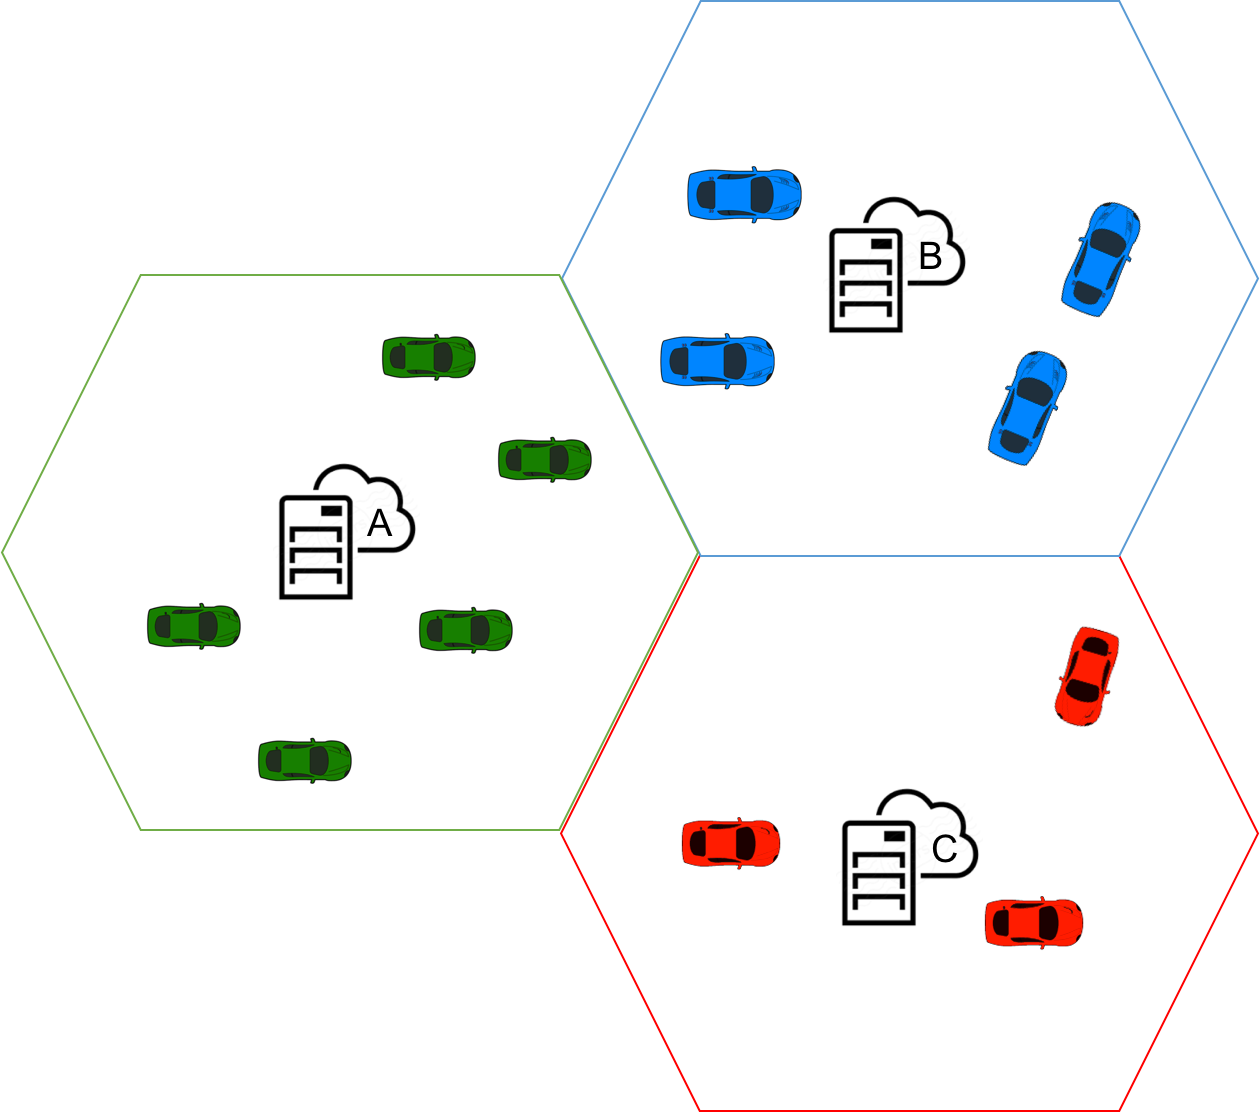
\includegraphics[width=0.75\linewidth]{images/car_rep}
\caption{Example Fog Computing Model}
\label{carrep}
\end{figure}



\subsection{Linear Mobility Pattern Prediction}
\label{background:model}
We propose a linear mobility prediction algorithm that uses just previous location and current location of a car to predict its future location. Assuming each car updates its location every $\theta$ seconds, when a car updates its location at time $t$, the corresponding fog server uses the car's previous location and timestamp to calculate the car's current speed and direction. The predicted location for the car will be the position of the car at time $t+\theta$ with current speed and direction. If the predicted location is outside of the current fog server's wireless range, then the algorithm will determine which server the car will travel to by finding the neighboring server that is the closest to the car’s predicted location. Figure \ref{carmodelrep} shows a graphical illustration of the prediction algorithm. 

\begin{figure}[ht!]
\centering
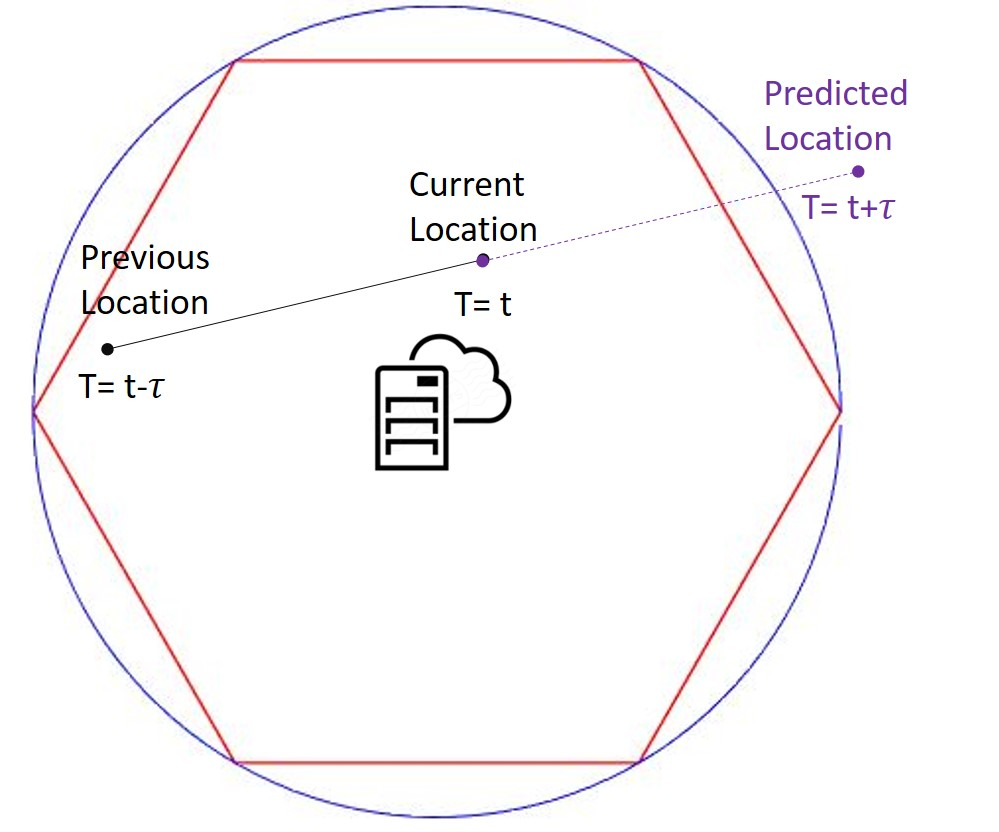
\includegraphics[width=0.5\linewidth]{images/car_model_rep}
\caption{Mobility Prediction Algorithm}
\label{carmodelrep}
\end{figure}


We test our linear prediction algorithm with real GPS data of taxis gathered in Rome, Italy\cite{romet}. The update period for the dataset is about 7 seconds. We divide up the region into a system with 7 fog nodes each with radius of 500 meters, as shown in Figure \ref{car7}. We use our linear prediction algorithm to keep track of the taxis' mobility pattern, and notify the system when the algorithm anticipates a taxi is leaving or entering the wireless coverage of the center fog node by predicting which of the 6 regions the taxi is heading toward or coming from. The result is shown in Figure \ref{RomeRes}, where the blue lines indicate correct predictions and red lines indicate incorrect predictions. We are able to obtain a 94.89\% accuracy as shown in Table \ref{cartable}. In the next section, we will present a task model based on the model presented in this section, and then develop an optimization problem formulation for load balancing that minimizes deadline misses and total runtime.


\begin{figure}[ht!]
\centering
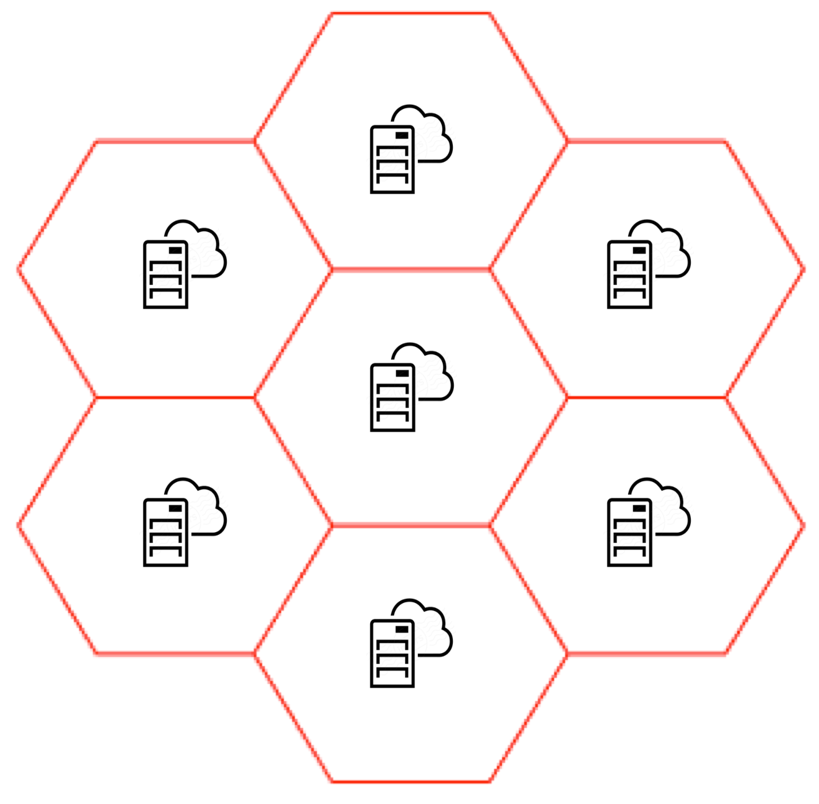
\includegraphics[width=0.5\linewidth]{images/car_7}
\caption{A Fog System with 7 Fog Nodes}
\label{car7}
\end{figure}


\begin{figure}[ht!]
\centering
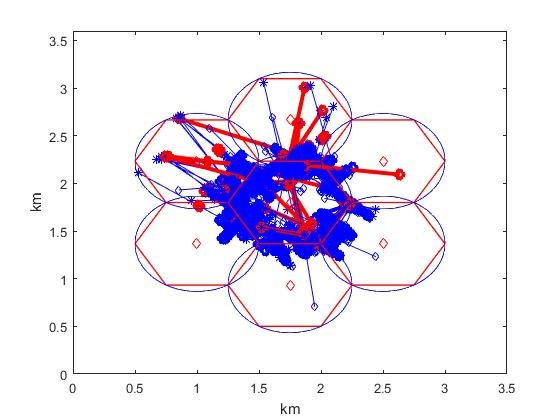
\includegraphics[width=1\linewidth]{images/car_res}
\caption{Linear Prediction Graphical Result}
\label{RomeRes}
\end{figure}


\begin{table}[h]
%\small
\caption{Linear Prediction Numerical Result}
\centering
\begin{tabular}{|m{4cm}|m{2cm}|}
	\hline
	Correct Preditction Count & 2505 \\ 
	\hline
	Total Prediction Count & 2640 \\ 
	\hline
	Accuracy & 94.89\% \\ \hline
\end{tabular}
\label{cartable}
\end{table}




















\section{Anchors Framework}


The main idea of Anchors is to dynamically allocate CPU resource to VMs by monitoring each VM’s real-time performance as shown in figure {meow}. In this section, we will go over each Anchors framework’s module in detail.


% \label{s4}
\subsection{Application's Real-Time Perfomance Feedback}

\subsubsection{Heartbeat API} 
We modified Heartbeat API to be used in Python. 
\subsubsection{Inter-Domain Communication}
We utilize Xenstore for VM to send its heartbeat information to Dom0.

\subsection{VM Monitor}

\subsubsection{Xen Scheduler}
RTDS and credit scheduler









\section{Controller Algorithm}

\subsubsection{AIMD}
range
\subsubsection{APID}
log
\subsubsection{Stride Scheduling}
meow



\section{Results and Discussion}
\label{s4}

\subsection{Experiment Setup}

Our simulation adopts the system with seven local fog servers as illustrated in Figure \ref{car7} and an additional cloud server. For fog servers, the link rate between server $i$ and server $j$, $B_{ij}$, is randomly drawn from between 16 and 64 tasks per second for $i\ne j$, or $\infty$ for $i=j$, the CPU frequency for server $j$, ${f_{j}}$, is randomly drawn from between 2700 MHz and 3600 MHz, and the capacity of server $j$, $C_{j}$,  is randomly drawn from between 10 and 35 tasks. For the remote cloud server, its initial tasks, $N_{cloud}$ is 0, $B_{icloud}$ is 4 tasks per second, ${f_{cloud}}$ is 4500MHz, and $C_{cloud}$ is $\infty$. For all servers, CPU cycles required per task, $x$, is set at 35 Mcycles, deadline for each task, $D$, is set at 0.5 second, and allowed processing time for each server, $\tau$, is 0.48 second. The system's parameters can be summarized in Table \ref{simvar}.

A taskset is generated by randomly selecting a number for $N_{i}$ from a range of integers which is shown in the first row in Table \ref{ntypes}. By varying the range of integers for $N_{i}$, we can create different loadings for the system. In each experiment, for the same type of loading, taskset generation is performed 100 times, and load balancing optimization is executed for each newly generated taskset. We record all the $N_{i}$ values and so each experiment can be run with the same tasksets. All the experiments were run in the machine with dual quadcore AMD Opteron 2.3 GHz with 16GB memory. The time it takes to execute linear prediction and to solve the optimization on that machine are both less than 0.01 second for all the experiments we run. So the overhead for mobility prediction and load balancing is less than 0.02 second, which is within the overhead budget, calculated by substracting deadline by allowed processing time, $D-\tau=0.5-0.48=0.02$.


\begin{table}[ht!]
\caption{Simulation Parameters}
\centering
\small
\begin{tabular}{| m{0.8cm} | m{1.6cm} | m{15em} |}
    \hline
    \multicolumn{3}{|l|}{\textbf{Simulation Parameters for the System}}\\
    \hline
    $k$ & 8 & Number of servers \\
    \hline
    $x$ & 35 & Number of CPU cycles required for each task (Mcycles)\\
    \hline
    $D$ & 0.5 & Deadline for all tasks (sec)\\
    \hline
    $\tau$ & 0.48 & Allowed processing time for each server (sec)\\
    \hline
    \multicolumn{3}{|l|}{\textbf{Simulation Parameters for Local Fog Servers}}\\
    \hline
    $N_{i}$ & see Table \ref{ntypes} & Number of initial tasks for server $i$\\
    \hline
    \multirow{2}{*}{$B_{ij}$} & [16,64] & Link rate between server $i$ and server $j$ for $i\ne j$ (tasks/sec) \\ \cline{2-3}
    & $\infty$ & Link rate between server $i$ and server $j$ for $i=j$ (tasks/sec) \\
    % $B_{ij}$ & [16,64] & Link rate between server $i$ and server $j$ (tasks/sec)\\
    \hline
    $C_{j}$ & [10,35] & Capacity of server $j$ (tasks)\\
    \hline
    $f_{j}$ & [2700,3600] & CPU frequency of server $j$ (MHz)\\
    \hline
    \multicolumn{3}{|l|}{\textbf{Simulation Parameters for Cloud Server}}\\
    \hline
    $N_{cloud}$ & 0 & Number of inital tasks for cloud server\\
    \hline
    $B_{icloud}$ & 4 & Link rate between server $i$ and cloud server (tasks/sec)\\
    \hline
    $C_{cloud}$ & $\infty$ & Capacity of cloud server (tasks)\\
    \hline
    $f_{cloud}$ & 4500 & CPU frequency of cloud server (MHz)\\
    \hline\hline
    \multicolumn{2}{|l|}{\textbf{Optimizing Variables}}\\
    \hline
    $n_{ij}$ & solved with optimization & Number of tasks distributed from server $i$ to server $j$\\
    \hline
\end{tabular}
\label{simvar}
\end{table}

\begin{table}[h]
\caption{Types of Workloads}
\small
\centering
\begin{tabular}{|m{1cm}|m{1cm}|m{1cm}|m{1cm}|m{1cm}|m{1cm}|}
    \hline
    Range for $N_{i}$ (tasks)& [10,26] & [10,28] & [10,30] & [10,32] & [10,34] \\ \hline
    Total number of tasks & 12687 & 13472 & 14143 & 14739 & 15051 \\ \hline
\end{tabular}
\label{ntypes}
\end{table}

\subsection{Deadline Misses vs Total Runtime}

In this experiment, we focus on the varying $v$, the weighing parameter in the optimization formulation presented. According to our objective function (\ref{opt_fstart}), a greater $v$ value should result in fewer deadline misses with higher total runtime. We verify such trend by running experiment with different $v$ and gather the results for deadline misses and total runtime respectively, as shown in Figure \ref{res_opt_vs_opt_md} and Figure \ref{res_opt_vs_opt_time}. From the figures, we observe that a larger $v$ does result in fewer deadline misses and higher total runtime.


\begin{figure}[h!]
\centering
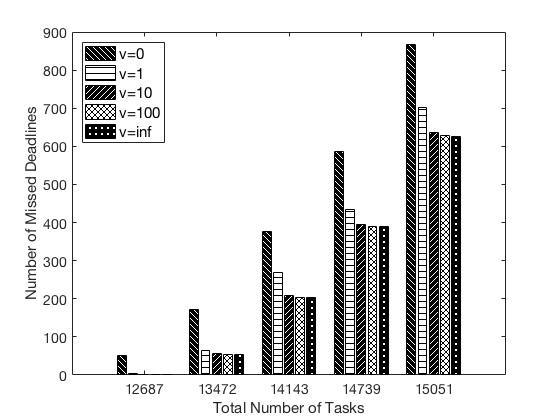
\includegraphics[width=1\linewidth]{images/res_opt_vs_opt_mdp}
\caption{Deadline Misses Comparison with Different $v$ }
\label{res_opt_vs_opt_md}
\end{figure}


\begin{figure}[h!]
\centering
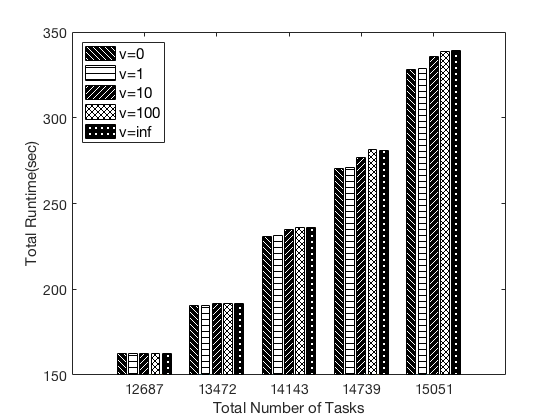
\includegraphics[width=1\linewidth]{images/res_opt_vs_opt_timep}
\caption{Total Runtime Comparison with Different $v$ }
\label{res_opt_vs_opt_time}
\end{figure}


\subsection{Comparison with Other Load Balancing Algorithms}



We compare our optimization result with local static, a simple load balancing method, and three other commonly used load balancing algorithms: weighted round robin, active monitoring and throttled load balancer\cite{wrr}\cite{amt}\cite{amt2}. In local static load balancing, each server with initial tasks exceed its capacity will transfer all the overloading tasks to the cloud server. Weighted round robin is implemented by assigning high weights for local servers that have not reached their maximum capacity. The cloud server will have a higher weight than a local server only when that server reaches its maximum capacity. Active monitoring load balancing is implemented by having each task assigned to the local server that has the highest remaining capacity, the algorithm will only assign to the cloud server when all the local servers are full. In the throttled load balancer, each task is assigned based on the most suitable server available, so the server with lowest completion time and has not reached its maximum capacity will be assigned with the new task. Again, a cloud server will be utilized only when none of the local servers are available. The comparisons are shown in Figure \ref{res_opt_vs_lb_ls_md} and Figure \ref{res_opt_vs_lb_ls_time}. Local static does not utilize any available local server so it is not surprising that local static is outperformed by more than 50\% in every case. On the other hand, our optimization has the least deadline misses and total runtime for every case. The numerical results for deadline misses is presented in Table \ref{good}. From Table \ref{good}, at a lighter load of 13472 tasks, our optimization outperforms throttled load balancer which has the second least deadline misses, by almost 50\%, but as the load of the system increases, the improvement brought by optimization starts to decrease. At the heaviest load of 15051 tasks, the improvment our optimization can bring drops to about 25\%. The reason being a heavy loaded system has fewer available options for task distributing, thus the potential for a better performance gets smaller as more load is added to the system.




 
% \begin{figure}[ht!]
% \centering
% 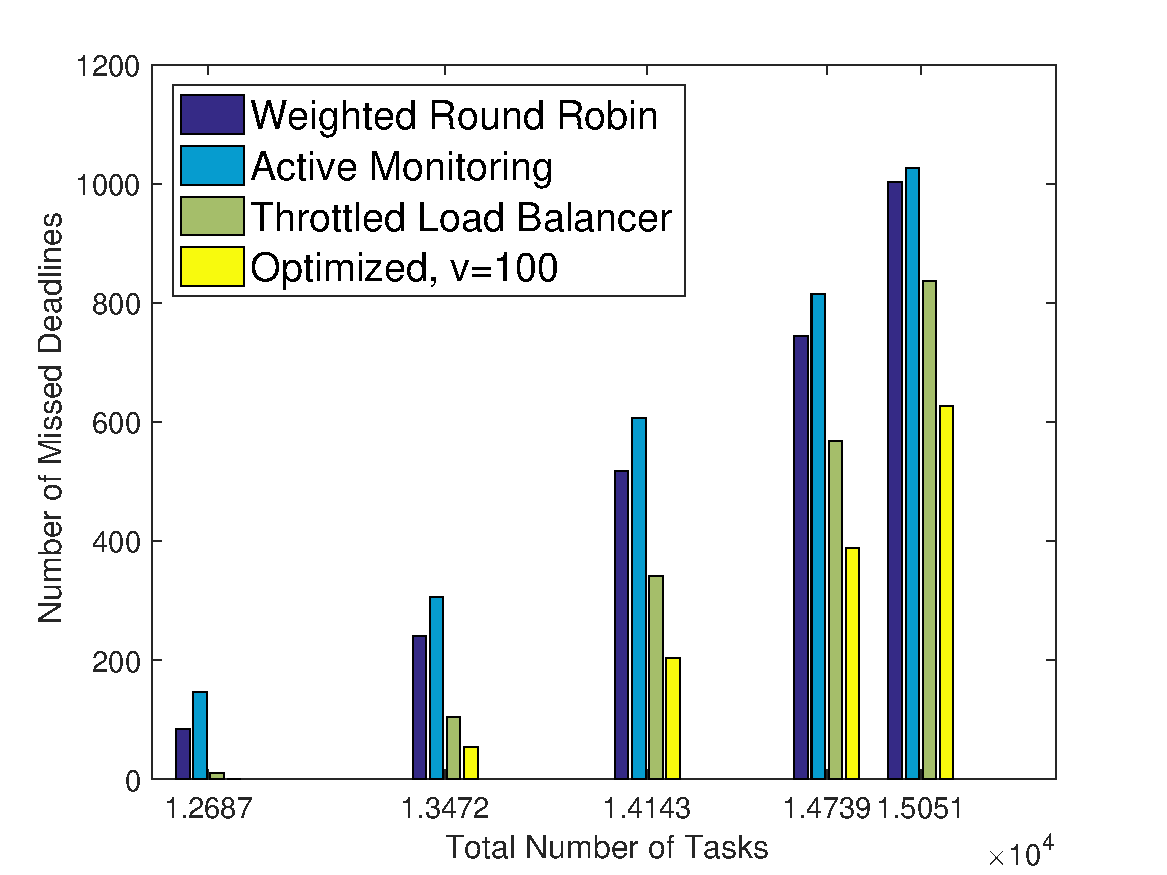
\includegraphics[width=1\linewidth]{images/res_opt_vs_lb_md}
% \caption{Deadline Misses Comparison with Other Load Balancing Algorithms}
% \label{res_opt_vs_lb_md}
% \end{figure}


% \begin{figure}[ht!]
% \centering
% 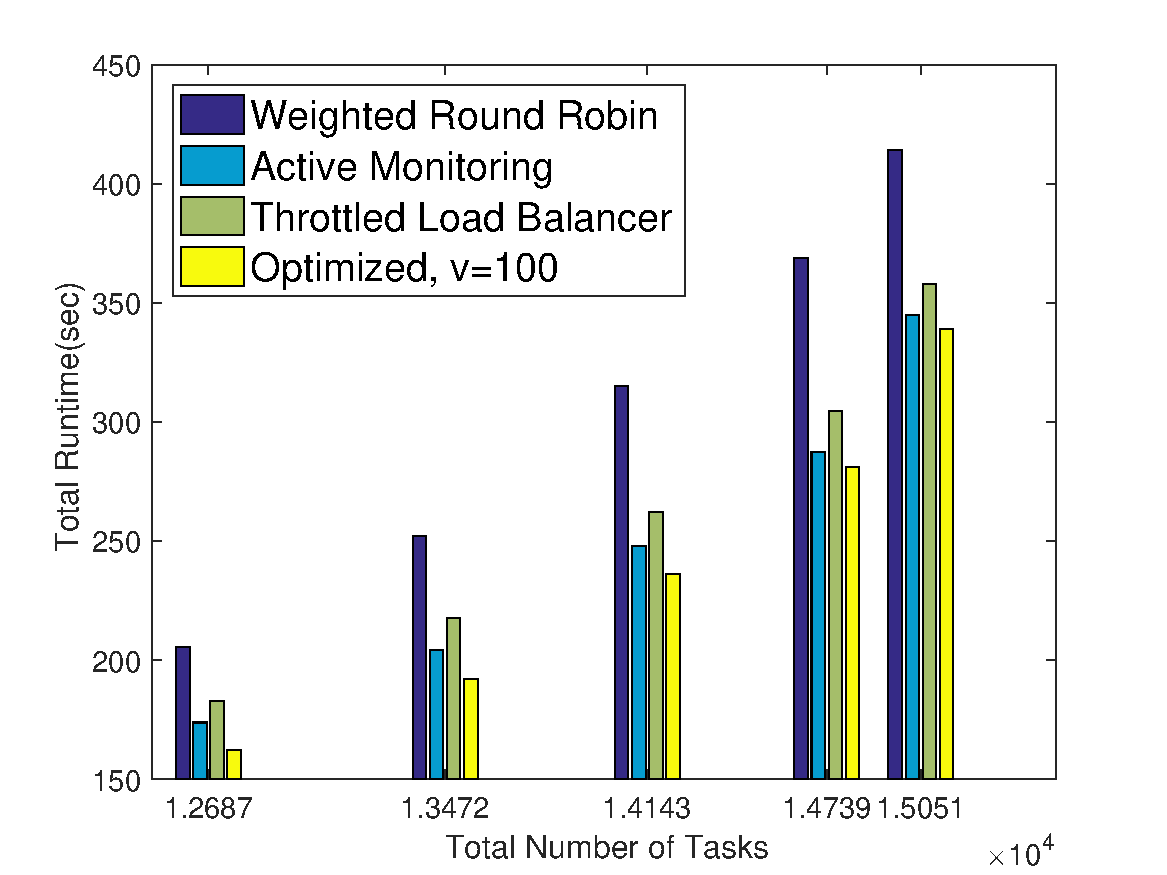
\includegraphics[width=1\linewidth]{images/res_opt_vs_lb_time}
% \caption{Total Runtime Comparison with Other Load Balancing Algorithms}
% \label{res_opt_vs_lb_time}
% \end{figure}

 
\begin{figure}[ht!]
\centering
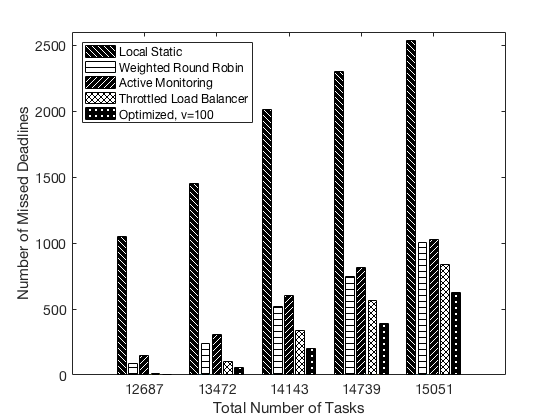
\includegraphics[width=1\linewidth]{images/res_opt_vs_lb_ls_mdp}
\caption{Deadline Misses Comparison with Other Load Balancing Algorithms}
\label{res_opt_vs_lb_ls_md}
\end{figure}


\begin{figure}[ht!]
\centering
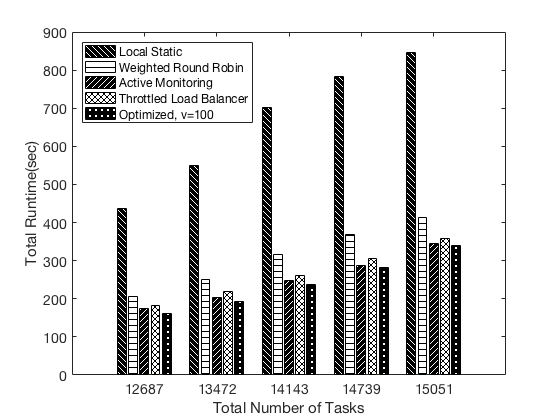
\includegraphics[width=1\linewidth]{images/res_opt_vs_lb_ls_timep}
\caption{Total Runtime Comparison with Other Load Balancing Algorithms}
\label{res_opt_vs_lb_ls_time}
\end{figure}

\begin{table}[h]
\small
\caption{Missed Deadlines Counts}
\centering
\begin{tabular}{|m{1.5cm}|m{0.75cm}|m{0.75cm}|m{0.75cm}|m{0.75cm}|m{0.75cm}|}
    \hline
    \textbf{Total number of tasks} & \textbf{12687} & \textbf{13472} & \textbf{14143} & \textbf{14739} & \textbf{15051} \\ 
    \hline
    Optimized, $v$=100 & 0 & 54 & 204 & 389 & 627 \\
    \hline
    Local Static & 1052 & 1454 & 2011 & 2300 & 2535 \\
    \hline
    Weighted Round Robin & 85 & 240 & 517 & 745& 1003 \\
    \hline
    Active Monitoring & 147 & 306 & 606 & 815& 1026 \\
    \hline
    Throttled Load Balancer & 11 & 104 & 341 & 568& 837 \\
    \hline
\end{tabular}
\label{good}
\end{table}

% \begin{table}[h]
% \small
% \caption{Missed Deadlines Counts}
% \centering
% \begin{tabular}{|m{1.5cm}|m{0.75cm}|m{0.75cm}|m{0.75cm}|m{0.75cm}|m{0.75cm}|}
%     \hline
%     \textbf{Total number of tasks} & \textbf{12687} & \textbf{13472} & \textbf{14143} & \textbf{14739} & \textbf{15051} \\ 
%     \hline
%     Optimized, $v$=100 & 0 & 54 & 204 & 389 & 627 \\
%     \hline
%     Local Static & 1052 & 1454 & 2011 & 2300 & 2535 \\
%     \hline
%     Weighted Round Robin & 85 & 240 & 517 & 745& 1003 \\
%     \hline
%     Active Monitoring & 147 & 306 & 606 & 815& 1026 \\
%     \hline
%     Throttled Load Balancer & 11 & 104 & 341 & 568& 837 \\
%     \hline
% \end{tabular}
% \label{good}
% \end{table}


% \begin{table}[h]
% \small
% \caption{Deadline Misses ratio - deadline misses/total tasks, $v$=100}
% \centering
% \begin{tabular}{|m{1.5cm}|m{0.75cm}|m{0.75cm}|m{0.75cm}|m{0.75cm}|m{0.75cm}|}
%     \hline
%     \textbf{Total number of tasks} & \textbf{12687} & \textbf{13472} & \textbf{14143} & \textbf{14739} & \textbf{15051} \\  
%     \hline
%     Optimized, $v$=100 & 0\% & .40\% & 1.44\% & 2.64\% & 4.17\% \\
%     \hline
%     Local Static & 8.29\% & 10.79\% & 14.2\% & 15.6\% & 16.8\% \\
%     \hline
%     Weighted Roung Robin & 0.67\% & 1.78\% & 3.66\% & 5.05\% & 6.66\% \\
%     \hline
%     Active Monitoring  & 1.16\% & 2.27\% & 4.28\% & 5.53\% & 6.82\% \\    
%     \hline
%     Thorttled Load Balancer & 0.087\% & 0.77\% & 2.41\% & 3.85\% & 5.56\% \\
%     \hline
% \end{tabular}
% \label{bad}
% \end{table}



% \begin{table}[h]
% \small
% \caption{Deadline Misses Comparison to Optimized \%, $v$=100}
% \centering
% \begin{tabular}{|m{1.5cm}|m{0.75cm}|m{0.75cm}|m{0.75cm}|m{0.75cm}|m{0.75cm}|}
%     \hline
%     \textbf{Total number of tasks} & \textbf{12687} & \textbf{13472} & \textbf{14143} & \textbf{14739} & \textbf{15051} \\ 
%     \hline
%     Local Static & 100\% & 96.3\% & 89.9\% & 83.1\% & 75.3\% \\
%     \hline
%     Weighted Roung Robin  & 100\% & 77.5\% & 60.5\% & 48.8\%& 37.5\% \\
%     \hline
%     Active Monitoring  & 100\% & 82.4\% & 66.3\% & 52.3\%& 38.9\% \\
%     \hline
%     Thorttled Load Balancer & 100\% & 48.1\% & 40.2\% & 31.5\%& 25.1\% \\
%     \hline
% \end{tabular}
% \label{best}
% \end{table}

















%\section{Results}
% \section{Discussion}
Expect about 2 pages.

% JP to lead.

This is the discussion that follows the results.  It's possible that I may
combine these two sections into a single session (results and discussion). This
is where we point out the differences in results - where individual hypervisors
started to trip up, what characteristics they exhibited, etc.


\section{Conclusion and Future Work}
\label{s5}



In this work, we propose a task scheduling model for connected car system in fog computing that brings task scheduling from device level to server level, which reduces the amount of computations required to perform load balancing. We also formulate a load balancing optimization problem that minimizes deadline misses and total runtime. We show that our optimization outperforms some common load balancing algorithms such as weighted round robin, active monitoring, and throttled load balancer. There are many potentials and ideas to expand on this topic including take energy consumption into consideration, vary the parameters dynamically, or implement applications with real workloads. We look forward to pursuing more research in this topic as the development of fog computing and connected car systems continues.


% Adjust this to balance last page if not using package
\IEEEtriggeratref{24}
\bibliography{socc2018}
\bibliographystyle{./IEEEtranBST/IEEEtran}

\end{document}

